\documentclass[11pt]{amsart}
\usepackage[a4paper,margin=1in]{geometry}
\usepackage{amssymb,amsmath,booktabs}
\usepackage{tikz}
\usepackage[font=small,labelfont=bf]{caption}
\usepackage[hidelinks]{hyperref}

\colorlet{copper}{orange!75!black}
\colorlet{inkmuted}{black!60}
\tikzset{thin/.style={line width=0.4pt}}

\newtheorem{theorem}{Theorem}
\newtheorem{proposition}[theorem]{Proposition}
\newtheorem{lemma}[theorem]{Lemma}
\theoremstyle{remark}
\newtheorem{remark}[theorem]{Remark}
\newtheorem{observation}[theorem]{Observation}

\title{The Cells of a Regular Polygon Are Small}
\author{Vamshi Jandhyala}
\address{London, United Kingdom}
\email{vamshi.jandhyala@gmail.com}

\begin{document}

\begin{abstract}
Draw every diagonal of a regular $n$-gon with side $1$. We show that every cell has area at most $C/n$ for an absolute constant $C$, except the central cell when $n$ is odd, which we compute exactly: its area tends to $\pi/16$. Since the triangles on the sides have area $\frac14\tan(\pi/n)$, the largest ordinary cell has area of order $1/n$, which answers the boundedness question in a MathOverflow thread. The proof traps each cell between diagonals in two independent directions, found as lattice points near a rational tangent to the curve of chords through a point. We also certify, in ball arithmetic, that the side triangles are not the largest cells: for every $n$ from $9$ to $60$ except $10,18,28,34,57$ some cell is strictly larger. The sharp constant remains open.
\end{abstract}

\maketitle

\section{The question}

Take a regular $n$-gon with side $1$ and draw all its diagonals. They cut the polygon into cells (Figure~\ref{fig:polygon}). How large can a cell be? The cells next to the sides are triangles of area $\frac14\tan(\pi/n)\approx\pi/(4n)$, and it is natural to guess that nothing is much bigger. A MathOverflow question asks for bounds on the largest cell~\cite{MO}, and, failing sharp bounds, whether $n$ times the largest area stays bounded; a twin question on Mathematics Stack Exchange asks the same~\cite{MSE}. Before reading on, look at the $9$-gon in Figure~\ref{fig:polygon}: is the blue side triangle the largest cell?

It is not, but it is the right size.

\begin{theorem}\label{thm:main}
There is an absolute constant $C$ such that, for every $n\ge4$, every cell of the regular $n$-gon with side $1$ and all diagonals drawn has area at most $C/n$, except the central cell when $n$ is odd.
\end{theorem}

\begin{proposition}\label{prop:central}
For odd $n\ge5$ the central cell is a regular $n$-gon with inradius $\bigl(4\cos\frac{\pi}{2n}\bigr)^{-1}$, so its area is
\[
\frac{n\tan(\pi/n)}{16\cos^2(\pi/2n)}\longrightarrow\frac{\pi}{16}.
\]
\end{proposition}

So the exception in Theorem~\ref{thm:main} is necessary, and for odd $n$ the central cell is the largest by far. Among the other cells the side triangles show that the bound $C/n$ is of the right order, but they are not the largest.

\begin{observation}\label{obs:largest}
For every $n$ with $9\le n\le60$ other than $10,18,28,34,57$, some cell other than the odd central cell has area strictly greater than $\frac14\tan(\pi/n)$. This is certified in ball arithmetic (Section~\ref{sec:largest}). At $n=31$ the certified cell has area at least $0.03903$ against $0.02542$ for a side triangle.
\end{observation}

\begin{figure}[ht]
\centering
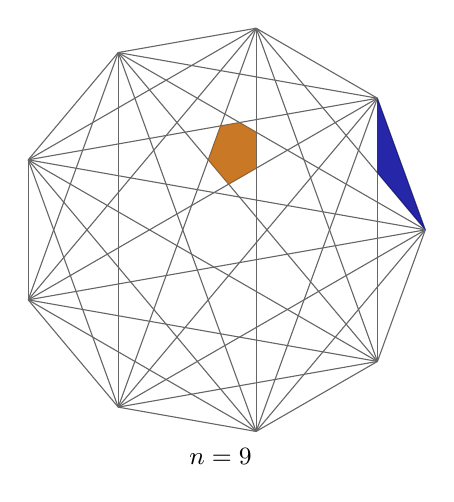
\begin{tikzpicture}[scale=1.7785]
\draw[inkmuted,line width=0.4pt] (1.4619,0.0000)--(1.1199,0.9397);
\draw[inkmuted,line width=0.4pt] (1.4619,0.0000)--(0.2539,1.4397);
\draw[inkmuted,line width=0.4pt] (1.4619,0.0000)--(-0.7310,1.2660);
\draw[inkmuted,line width=0.4pt] (1.4619,0.0000)--(-1.3737,0.5000);
\draw[inkmuted,line width=0.4pt] (1.4619,0.0000)--(-1.3737,-0.5000);
\draw[inkmuted,line width=0.4pt] (1.4619,0.0000)--(-0.7310,-1.2660);
\draw[inkmuted,line width=0.4pt] (1.4619,0.0000)--(0.2539,-1.4397);
\draw[inkmuted,line width=0.4pt] (1.4619,0.0000)--(1.1199,-0.9397);
\draw[inkmuted,line width=0.4pt] (1.1199,0.9397)--(0.2539,1.4397);
\draw[inkmuted,line width=0.4pt] (1.1199,0.9397)--(-0.7310,1.2660);
\draw[inkmuted,line width=0.4pt] (1.1199,0.9397)--(-1.3737,0.5000);
\draw[inkmuted,line width=0.4pt] (1.1199,0.9397)--(-1.3737,-0.5000);
\draw[inkmuted,line width=0.4pt] (1.1199,0.9397)--(-0.7310,-1.2660);
\draw[inkmuted,line width=0.4pt] (1.1199,0.9397)--(0.2539,-1.4397);
\draw[inkmuted,line width=0.4pt] (1.1199,0.9397)--(1.1199,-0.9397);
\draw[inkmuted,line width=0.4pt] (0.2539,1.4397)--(-0.7310,1.2660);
\draw[inkmuted,line width=0.4pt] (0.2539,1.4397)--(-1.3737,0.5000);
\draw[inkmuted,line width=0.4pt] (0.2539,1.4397)--(-1.3737,-0.5000);
\draw[inkmuted,line width=0.4pt] (0.2539,1.4397)--(-0.7310,-1.2660);
\draw[inkmuted,line width=0.4pt] (0.2539,1.4397)--(0.2539,-1.4397);
\draw[inkmuted,line width=0.4pt] (0.2539,1.4397)--(1.1199,-0.9397);
\draw[inkmuted,line width=0.4pt] (-0.7310,1.2660)--(-1.3737,0.5000);
\draw[inkmuted,line width=0.4pt] (-0.7310,1.2660)--(-1.3737,-0.5000);
\draw[inkmuted,line width=0.4pt] (-0.7310,1.2660)--(-0.7310,-1.2660);
\draw[inkmuted,line width=0.4pt] (-0.7310,1.2660)--(0.2539,-1.4397);
\draw[inkmuted,line width=0.4pt] (-0.7310,1.2660)--(1.1199,-0.9397);
\draw[inkmuted,line width=0.4pt] (-1.3737,0.5000)--(-1.3737,-0.5000);
\draw[inkmuted,line width=0.4pt] (-1.3737,0.5000)--(-0.7310,-1.2660);
\draw[inkmuted,line width=0.4pt] (-1.3737,0.5000)--(0.2539,-1.4397);
\draw[inkmuted,line width=0.4pt] (-1.3737,0.5000)--(1.1199,-0.9397);
\draw[inkmuted,line width=0.4pt] (-1.3737,-0.5000)--(-0.7310,-1.2660);
\draw[inkmuted,line width=0.4pt] (-1.3737,-0.5000)--(0.2539,-1.4397);
\draw[inkmuted,line width=0.4pt] (-1.3737,-0.5000)--(1.1199,-0.9397);
\draw[inkmuted,line width=0.4pt] (-0.7310,-1.2660)--(0.2539,-1.4397);
\draw[inkmuted,line width=0.4pt] (-0.7310,-1.2660)--(1.1199,-0.9397);
\draw[inkmuted,line width=0.4pt] (0.2539,-1.4397)--(1.1199,-0.9397);
\fill[blue!60!black,opacity=0.85] (1.1199,0.9397) -- (1.4619,0.0000) -- (1.1199,0.4076) -- cycle;
\fill[copper,opacity=0.85] (0.1351,0.7660) -- (0.2539,0.6975) -- (0.2539,0.4397) -- (0.0575,0.3264) -- (-0.0882,0.5000) -- (-0.0000,0.7422) -- cycle;
\node[below] at (0,-1.491) {\small $n=9$};
\end{tikzpicture}
\hspace{1.2em}
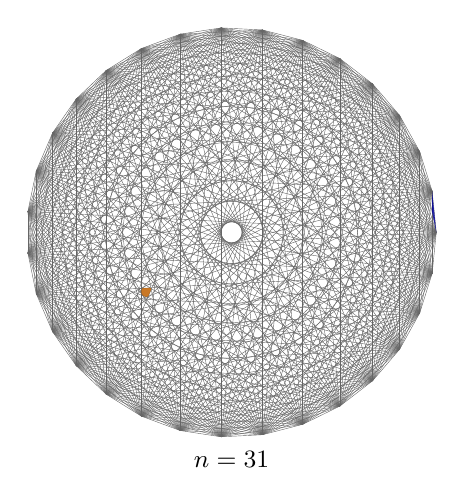
\begin{tikzpicture}[scale=0.5261]
\draw[inkmuted,line width=0.15pt] (4.9423,0.0000)--(4.8411,0.9949);
\draw[inkmuted,line width=0.15pt] (4.9423,0.0000)--(4.5417,1.9490);
\draw[inkmuted,line width=0.15pt] (4.9423,0.0000)--(4.0564,2.8234);
\draw[inkmuted,line width=0.15pt] (4.9423,0.0000)--(3.4051,3.5821);
\draw[inkmuted,line width=0.15pt] (4.9423,0.0000)--(2.6143,4.1942);
\draw[inkmuted,line width=0.15pt] (4.9423,0.0000)--(1.7165,4.6346);
\draw[inkmuted,line width=0.15pt] (4.9423,0.0000)--(0.7484,4.8853);
\draw[inkmuted,line width=0.15pt] (4.9423,0.0000)--(-0.2503,4.9359);
\draw[inkmuted,line width=0.15pt] (4.9423,0.0000)--(-1.2388,4.7845);
\draw[inkmuted,line width=0.15pt] (4.9423,0.0000)--(-2.1765,4.4372);
\draw[inkmuted,line width=0.15pt] (4.9423,0.0000)--(-3.0252,3.9082);
\draw[inkmuted,line width=0.15pt] (4.9423,0.0000)--(-3.7500,3.2193);
\draw[inkmuted,line width=0.15pt] (4.9423,0.0000)--(-4.3212,2.3985);
\draw[inkmuted,line width=0.15pt] (4.9423,0.0000)--(-4.7156,1.4795);
\draw[inkmuted,line width=0.15pt] (4.9423,0.0000)--(-4.9169,0.5000);
\draw[inkmuted,line width=0.15pt] (4.9423,0.0000)--(-4.9169,-0.5000);
\draw[inkmuted,line width=0.15pt] (4.9423,0.0000)--(-4.7156,-1.4795);
\draw[inkmuted,line width=0.15pt] (4.9423,0.0000)--(-4.3212,-2.3985);
\draw[inkmuted,line width=0.15pt] (4.9423,0.0000)--(-3.7500,-3.2193);
\draw[inkmuted,line width=0.15pt] (4.9423,0.0000)--(-3.0252,-3.9082);
\draw[inkmuted,line width=0.15pt] (4.9423,0.0000)--(-2.1765,-4.4372);
\draw[inkmuted,line width=0.15pt] (4.9423,0.0000)--(-1.2388,-4.7845);
\draw[inkmuted,line width=0.15pt] (4.9423,0.0000)--(-0.2503,-4.9359);
\draw[inkmuted,line width=0.15pt] (4.9423,0.0000)--(0.7484,-4.8853);
\draw[inkmuted,line width=0.15pt] (4.9423,0.0000)--(1.7165,-4.6346);
\draw[inkmuted,line width=0.15pt] (4.9423,0.0000)--(2.6143,-4.1942);
\draw[inkmuted,line width=0.15pt] (4.9423,0.0000)--(3.4051,-3.5821);
\draw[inkmuted,line width=0.15pt] (4.9423,0.0000)--(4.0564,-2.8234);
\draw[inkmuted,line width=0.15pt] (4.9423,0.0000)--(4.5417,-1.9490);
\draw[inkmuted,line width=0.15pt] (4.9423,0.0000)--(4.8411,-0.9949);
\draw[inkmuted,line width=0.15pt] (4.8411,0.9949)--(4.5417,1.9490);
\draw[inkmuted,line width=0.15pt] (4.8411,0.9949)--(4.0564,2.8234);
\draw[inkmuted,line width=0.15pt] (4.8411,0.9949)--(3.4051,3.5821);
\draw[inkmuted,line width=0.15pt] (4.8411,0.9949)--(2.6143,4.1942);
\draw[inkmuted,line width=0.15pt] (4.8411,0.9949)--(1.7165,4.6346);
\draw[inkmuted,line width=0.15pt] (4.8411,0.9949)--(0.7484,4.8853);
\draw[inkmuted,line width=0.15pt] (4.8411,0.9949)--(-0.2503,4.9359);
\draw[inkmuted,line width=0.15pt] (4.8411,0.9949)--(-1.2388,4.7845);
\draw[inkmuted,line width=0.15pt] (4.8411,0.9949)--(-2.1765,4.4372);
\draw[inkmuted,line width=0.15pt] (4.8411,0.9949)--(-3.0252,3.9082);
\draw[inkmuted,line width=0.15pt] (4.8411,0.9949)--(-3.7500,3.2193);
\draw[inkmuted,line width=0.15pt] (4.8411,0.9949)--(-4.3212,2.3985);
\draw[inkmuted,line width=0.15pt] (4.8411,0.9949)--(-4.7156,1.4795);
\draw[inkmuted,line width=0.15pt] (4.8411,0.9949)--(-4.9169,0.5000);
\draw[inkmuted,line width=0.15pt] (4.8411,0.9949)--(-4.9169,-0.5000);
\draw[inkmuted,line width=0.15pt] (4.8411,0.9949)--(-4.7156,-1.4795);
\draw[inkmuted,line width=0.15pt] (4.8411,0.9949)--(-4.3212,-2.3985);
\draw[inkmuted,line width=0.15pt] (4.8411,0.9949)--(-3.7500,-3.2193);
\draw[inkmuted,line width=0.15pt] (4.8411,0.9949)--(-3.0252,-3.9082);
\draw[inkmuted,line width=0.15pt] (4.8411,0.9949)--(-2.1765,-4.4372);
\draw[inkmuted,line width=0.15pt] (4.8411,0.9949)--(-1.2388,-4.7845);
\draw[inkmuted,line width=0.15pt] (4.8411,0.9949)--(-0.2503,-4.9359);
\draw[inkmuted,line width=0.15pt] (4.8411,0.9949)--(0.7484,-4.8853);
\draw[inkmuted,line width=0.15pt] (4.8411,0.9949)--(1.7165,-4.6346);
\draw[inkmuted,line width=0.15pt] (4.8411,0.9949)--(2.6143,-4.1942);
\draw[inkmuted,line width=0.15pt] (4.8411,0.9949)--(3.4051,-3.5821);
\draw[inkmuted,line width=0.15pt] (4.8411,0.9949)--(4.0564,-2.8234);
\draw[inkmuted,line width=0.15pt] (4.8411,0.9949)--(4.5417,-1.9490);
\draw[inkmuted,line width=0.15pt] (4.8411,0.9949)--(4.8411,-0.9949);
\draw[inkmuted,line width=0.15pt] (4.5417,1.9490)--(4.0564,2.8234);
\draw[inkmuted,line width=0.15pt] (4.5417,1.9490)--(3.4051,3.5821);
\draw[inkmuted,line width=0.15pt] (4.5417,1.9490)--(2.6143,4.1942);
\draw[inkmuted,line width=0.15pt] (4.5417,1.9490)--(1.7165,4.6346);
\draw[inkmuted,line width=0.15pt] (4.5417,1.9490)--(0.7484,4.8853);
\draw[inkmuted,line width=0.15pt] (4.5417,1.9490)--(-0.2503,4.9359);
\draw[inkmuted,line width=0.15pt] (4.5417,1.9490)--(-1.2388,4.7845);
\draw[inkmuted,line width=0.15pt] (4.5417,1.9490)--(-2.1765,4.4372);
\draw[inkmuted,line width=0.15pt] (4.5417,1.9490)--(-3.0252,3.9082);
\draw[inkmuted,line width=0.15pt] (4.5417,1.9490)--(-3.7500,3.2193);
\draw[inkmuted,line width=0.15pt] (4.5417,1.9490)--(-4.3212,2.3985);
\draw[inkmuted,line width=0.15pt] (4.5417,1.9490)--(-4.7156,1.4795);
\draw[inkmuted,line width=0.15pt] (4.5417,1.9490)--(-4.9169,0.5000);
\draw[inkmuted,line width=0.15pt] (4.5417,1.9490)--(-4.9169,-0.5000);
\draw[inkmuted,line width=0.15pt] (4.5417,1.9490)--(-4.7156,-1.4795);
\draw[inkmuted,line width=0.15pt] (4.5417,1.9490)--(-4.3212,-2.3985);
\draw[inkmuted,line width=0.15pt] (4.5417,1.9490)--(-3.7500,-3.2193);
\draw[inkmuted,line width=0.15pt] (4.5417,1.9490)--(-3.0252,-3.9082);
\draw[inkmuted,line width=0.15pt] (4.5417,1.9490)--(-2.1765,-4.4372);
\draw[inkmuted,line width=0.15pt] (4.5417,1.9490)--(-1.2388,-4.7845);
\draw[inkmuted,line width=0.15pt] (4.5417,1.9490)--(-0.2503,-4.9359);
\draw[inkmuted,line width=0.15pt] (4.5417,1.9490)--(0.7484,-4.8853);
\draw[inkmuted,line width=0.15pt] (4.5417,1.9490)--(1.7165,-4.6346);
\draw[inkmuted,line width=0.15pt] (4.5417,1.9490)--(2.6143,-4.1942);
\draw[inkmuted,line width=0.15pt] (4.5417,1.9490)--(3.4051,-3.5821);
\draw[inkmuted,line width=0.15pt] (4.5417,1.9490)--(4.0564,-2.8234);
\draw[inkmuted,line width=0.15pt] (4.5417,1.9490)--(4.5417,-1.9490);
\draw[inkmuted,line width=0.15pt] (4.5417,1.9490)--(4.8411,-0.9949);
\draw[inkmuted,line width=0.15pt] (4.0564,2.8234)--(3.4051,3.5821);
\draw[inkmuted,line width=0.15pt] (4.0564,2.8234)--(2.6143,4.1942);
\draw[inkmuted,line width=0.15pt] (4.0564,2.8234)--(1.7165,4.6346);
\draw[inkmuted,line width=0.15pt] (4.0564,2.8234)--(0.7484,4.8853);
\draw[inkmuted,line width=0.15pt] (4.0564,2.8234)--(-0.2503,4.9359);
\draw[inkmuted,line width=0.15pt] (4.0564,2.8234)--(-1.2388,4.7845);
\draw[inkmuted,line width=0.15pt] (4.0564,2.8234)--(-2.1765,4.4372);
\draw[inkmuted,line width=0.15pt] (4.0564,2.8234)--(-3.0252,3.9082);
\draw[inkmuted,line width=0.15pt] (4.0564,2.8234)--(-3.7500,3.2193);
\draw[inkmuted,line width=0.15pt] (4.0564,2.8234)--(-4.3212,2.3985);
\draw[inkmuted,line width=0.15pt] (4.0564,2.8234)--(-4.7156,1.4795);
\draw[inkmuted,line width=0.15pt] (4.0564,2.8234)--(-4.9169,0.5000);
\draw[inkmuted,line width=0.15pt] (4.0564,2.8234)--(-4.9169,-0.5000);
\draw[inkmuted,line width=0.15pt] (4.0564,2.8234)--(-4.7156,-1.4795);
\draw[inkmuted,line width=0.15pt] (4.0564,2.8234)--(-4.3212,-2.3985);
\draw[inkmuted,line width=0.15pt] (4.0564,2.8234)--(-3.7500,-3.2193);
\draw[inkmuted,line width=0.15pt] (4.0564,2.8234)--(-3.0252,-3.9082);
\draw[inkmuted,line width=0.15pt] (4.0564,2.8234)--(-2.1765,-4.4372);
\draw[inkmuted,line width=0.15pt] (4.0564,2.8234)--(-1.2388,-4.7845);
\draw[inkmuted,line width=0.15pt] (4.0564,2.8234)--(-0.2503,-4.9359);
\draw[inkmuted,line width=0.15pt] (4.0564,2.8234)--(0.7484,-4.8853);
\draw[inkmuted,line width=0.15pt] (4.0564,2.8234)--(1.7165,-4.6346);
\draw[inkmuted,line width=0.15pt] (4.0564,2.8234)--(2.6143,-4.1942);
\draw[inkmuted,line width=0.15pt] (4.0564,2.8234)--(3.4051,-3.5821);
\draw[inkmuted,line width=0.15pt] (4.0564,2.8234)--(4.0564,-2.8234);
\draw[inkmuted,line width=0.15pt] (4.0564,2.8234)--(4.5417,-1.9490);
\draw[inkmuted,line width=0.15pt] (4.0564,2.8234)--(4.8411,-0.9949);
\draw[inkmuted,line width=0.15pt] (3.4051,3.5821)--(2.6143,4.1942);
\draw[inkmuted,line width=0.15pt] (3.4051,3.5821)--(1.7165,4.6346);
\draw[inkmuted,line width=0.15pt] (3.4051,3.5821)--(0.7484,4.8853);
\draw[inkmuted,line width=0.15pt] (3.4051,3.5821)--(-0.2503,4.9359);
\draw[inkmuted,line width=0.15pt] (3.4051,3.5821)--(-1.2388,4.7845);
\draw[inkmuted,line width=0.15pt] (3.4051,3.5821)--(-2.1765,4.4372);
\draw[inkmuted,line width=0.15pt] (3.4051,3.5821)--(-3.0252,3.9082);
\draw[inkmuted,line width=0.15pt] (3.4051,3.5821)--(-3.7500,3.2193);
\draw[inkmuted,line width=0.15pt] (3.4051,3.5821)--(-4.3212,2.3985);
\draw[inkmuted,line width=0.15pt] (3.4051,3.5821)--(-4.7156,1.4795);
\draw[inkmuted,line width=0.15pt] (3.4051,3.5821)--(-4.9169,0.5000);
\draw[inkmuted,line width=0.15pt] (3.4051,3.5821)--(-4.9169,-0.5000);
\draw[inkmuted,line width=0.15pt] (3.4051,3.5821)--(-4.7156,-1.4795);
\draw[inkmuted,line width=0.15pt] (3.4051,3.5821)--(-4.3212,-2.3985);
\draw[inkmuted,line width=0.15pt] (3.4051,3.5821)--(-3.7500,-3.2193);
\draw[inkmuted,line width=0.15pt] (3.4051,3.5821)--(-3.0252,-3.9082);
\draw[inkmuted,line width=0.15pt] (3.4051,3.5821)--(-2.1765,-4.4372);
\draw[inkmuted,line width=0.15pt] (3.4051,3.5821)--(-1.2388,-4.7845);
\draw[inkmuted,line width=0.15pt] (3.4051,3.5821)--(-0.2503,-4.9359);
\draw[inkmuted,line width=0.15pt] (3.4051,3.5821)--(0.7484,-4.8853);
\draw[inkmuted,line width=0.15pt] (3.4051,3.5821)--(1.7165,-4.6346);
\draw[inkmuted,line width=0.15pt] (3.4051,3.5821)--(2.6143,-4.1942);
\draw[inkmuted,line width=0.15pt] (3.4051,3.5821)--(3.4051,-3.5821);
\draw[inkmuted,line width=0.15pt] (3.4051,3.5821)--(4.0564,-2.8234);
\draw[inkmuted,line width=0.15pt] (3.4051,3.5821)--(4.5417,-1.9490);
\draw[inkmuted,line width=0.15pt] (3.4051,3.5821)--(4.8411,-0.9949);
\draw[inkmuted,line width=0.15pt] (2.6143,4.1942)--(1.7165,4.6346);
\draw[inkmuted,line width=0.15pt] (2.6143,4.1942)--(0.7484,4.8853);
\draw[inkmuted,line width=0.15pt] (2.6143,4.1942)--(-0.2503,4.9359);
\draw[inkmuted,line width=0.15pt] (2.6143,4.1942)--(-1.2388,4.7845);
\draw[inkmuted,line width=0.15pt] (2.6143,4.1942)--(-2.1765,4.4372);
\draw[inkmuted,line width=0.15pt] (2.6143,4.1942)--(-3.0252,3.9082);
\draw[inkmuted,line width=0.15pt] (2.6143,4.1942)--(-3.7500,3.2193);
\draw[inkmuted,line width=0.15pt] (2.6143,4.1942)--(-4.3212,2.3985);
\draw[inkmuted,line width=0.15pt] (2.6143,4.1942)--(-4.7156,1.4795);
\draw[inkmuted,line width=0.15pt] (2.6143,4.1942)--(-4.9169,0.5000);
\draw[inkmuted,line width=0.15pt] (2.6143,4.1942)--(-4.9169,-0.5000);
\draw[inkmuted,line width=0.15pt] (2.6143,4.1942)--(-4.7156,-1.4795);
\draw[inkmuted,line width=0.15pt] (2.6143,4.1942)--(-4.3212,-2.3985);
\draw[inkmuted,line width=0.15pt] (2.6143,4.1942)--(-3.7500,-3.2193);
\draw[inkmuted,line width=0.15pt] (2.6143,4.1942)--(-3.0252,-3.9082);
\draw[inkmuted,line width=0.15pt] (2.6143,4.1942)--(-2.1765,-4.4372);
\draw[inkmuted,line width=0.15pt] (2.6143,4.1942)--(-1.2388,-4.7845);
\draw[inkmuted,line width=0.15pt] (2.6143,4.1942)--(-0.2503,-4.9359);
\draw[inkmuted,line width=0.15pt] (2.6143,4.1942)--(0.7484,-4.8853);
\draw[inkmuted,line width=0.15pt] (2.6143,4.1942)--(1.7165,-4.6346);
\draw[inkmuted,line width=0.15pt] (2.6143,4.1942)--(2.6143,-4.1942);
\draw[inkmuted,line width=0.15pt] (2.6143,4.1942)--(3.4051,-3.5821);
\draw[inkmuted,line width=0.15pt] (2.6143,4.1942)--(4.0564,-2.8234);
\draw[inkmuted,line width=0.15pt] (2.6143,4.1942)--(4.5417,-1.9490);
\draw[inkmuted,line width=0.15pt] (2.6143,4.1942)--(4.8411,-0.9949);
\draw[inkmuted,line width=0.15pt] (1.7165,4.6346)--(0.7484,4.8853);
\draw[inkmuted,line width=0.15pt] (1.7165,4.6346)--(-0.2503,4.9359);
\draw[inkmuted,line width=0.15pt] (1.7165,4.6346)--(-1.2388,4.7845);
\draw[inkmuted,line width=0.15pt] (1.7165,4.6346)--(-2.1765,4.4372);
\draw[inkmuted,line width=0.15pt] (1.7165,4.6346)--(-3.0252,3.9082);
\draw[inkmuted,line width=0.15pt] (1.7165,4.6346)--(-3.7500,3.2193);
\draw[inkmuted,line width=0.15pt] (1.7165,4.6346)--(-4.3212,2.3985);
\draw[inkmuted,line width=0.15pt] (1.7165,4.6346)--(-4.7156,1.4795);
\draw[inkmuted,line width=0.15pt] (1.7165,4.6346)--(-4.9169,0.5000);
\draw[inkmuted,line width=0.15pt] (1.7165,4.6346)--(-4.9169,-0.5000);
\draw[inkmuted,line width=0.15pt] (1.7165,4.6346)--(-4.7156,-1.4795);
\draw[inkmuted,line width=0.15pt] (1.7165,4.6346)--(-4.3212,-2.3985);
\draw[inkmuted,line width=0.15pt] (1.7165,4.6346)--(-3.7500,-3.2193);
\draw[inkmuted,line width=0.15pt] (1.7165,4.6346)--(-3.0252,-3.9082);
\draw[inkmuted,line width=0.15pt] (1.7165,4.6346)--(-2.1765,-4.4372);
\draw[inkmuted,line width=0.15pt] (1.7165,4.6346)--(-1.2388,-4.7845);
\draw[inkmuted,line width=0.15pt] (1.7165,4.6346)--(-0.2503,-4.9359);
\draw[inkmuted,line width=0.15pt] (1.7165,4.6346)--(0.7484,-4.8853);
\draw[inkmuted,line width=0.15pt] (1.7165,4.6346)--(1.7165,-4.6346);
\draw[inkmuted,line width=0.15pt] (1.7165,4.6346)--(2.6143,-4.1942);
\draw[inkmuted,line width=0.15pt] (1.7165,4.6346)--(3.4051,-3.5821);
\draw[inkmuted,line width=0.15pt] (1.7165,4.6346)--(4.0564,-2.8234);
\draw[inkmuted,line width=0.15pt] (1.7165,4.6346)--(4.5417,-1.9490);
\draw[inkmuted,line width=0.15pt] (1.7165,4.6346)--(4.8411,-0.9949);
\draw[inkmuted,line width=0.15pt] (0.7484,4.8853)--(-0.2503,4.9359);
\draw[inkmuted,line width=0.15pt] (0.7484,4.8853)--(-1.2388,4.7845);
\draw[inkmuted,line width=0.15pt] (0.7484,4.8853)--(-2.1765,4.4372);
\draw[inkmuted,line width=0.15pt] (0.7484,4.8853)--(-3.0252,3.9082);
\draw[inkmuted,line width=0.15pt] (0.7484,4.8853)--(-3.7500,3.2193);
\draw[inkmuted,line width=0.15pt] (0.7484,4.8853)--(-4.3212,2.3985);
\draw[inkmuted,line width=0.15pt] (0.7484,4.8853)--(-4.7156,1.4795);
\draw[inkmuted,line width=0.15pt] (0.7484,4.8853)--(-4.9169,0.5000);
\draw[inkmuted,line width=0.15pt] (0.7484,4.8853)--(-4.9169,-0.5000);
\draw[inkmuted,line width=0.15pt] (0.7484,4.8853)--(-4.7156,-1.4795);
\draw[inkmuted,line width=0.15pt] (0.7484,4.8853)--(-4.3212,-2.3985);
\draw[inkmuted,line width=0.15pt] (0.7484,4.8853)--(-3.7500,-3.2193);
\draw[inkmuted,line width=0.15pt] (0.7484,4.8853)--(-3.0252,-3.9082);
\draw[inkmuted,line width=0.15pt] (0.7484,4.8853)--(-2.1765,-4.4372);
\draw[inkmuted,line width=0.15pt] (0.7484,4.8853)--(-1.2388,-4.7845);
\draw[inkmuted,line width=0.15pt] (0.7484,4.8853)--(-0.2503,-4.9359);
\draw[inkmuted,line width=0.15pt] (0.7484,4.8853)--(0.7484,-4.8853);
\draw[inkmuted,line width=0.15pt] (0.7484,4.8853)--(1.7165,-4.6346);
\draw[inkmuted,line width=0.15pt] (0.7484,4.8853)--(2.6143,-4.1942);
\draw[inkmuted,line width=0.15pt] (0.7484,4.8853)--(3.4051,-3.5821);
\draw[inkmuted,line width=0.15pt] (0.7484,4.8853)--(4.0564,-2.8234);
\draw[inkmuted,line width=0.15pt] (0.7484,4.8853)--(4.5417,-1.9490);
\draw[inkmuted,line width=0.15pt] (0.7484,4.8853)--(4.8411,-0.9949);
\draw[inkmuted,line width=0.15pt] (-0.2503,4.9359)--(-1.2388,4.7845);
\draw[inkmuted,line width=0.15pt] (-0.2503,4.9359)--(-2.1765,4.4372);
\draw[inkmuted,line width=0.15pt] (-0.2503,4.9359)--(-3.0252,3.9082);
\draw[inkmuted,line width=0.15pt] (-0.2503,4.9359)--(-3.7500,3.2193);
\draw[inkmuted,line width=0.15pt] (-0.2503,4.9359)--(-4.3212,2.3985);
\draw[inkmuted,line width=0.15pt] (-0.2503,4.9359)--(-4.7156,1.4795);
\draw[inkmuted,line width=0.15pt] (-0.2503,4.9359)--(-4.9169,0.5000);
\draw[inkmuted,line width=0.15pt] (-0.2503,4.9359)--(-4.9169,-0.5000);
\draw[inkmuted,line width=0.15pt] (-0.2503,4.9359)--(-4.7156,-1.4795);
\draw[inkmuted,line width=0.15pt] (-0.2503,4.9359)--(-4.3212,-2.3985);
\draw[inkmuted,line width=0.15pt] (-0.2503,4.9359)--(-3.7500,-3.2193);
\draw[inkmuted,line width=0.15pt] (-0.2503,4.9359)--(-3.0252,-3.9082);
\draw[inkmuted,line width=0.15pt] (-0.2503,4.9359)--(-2.1765,-4.4372);
\draw[inkmuted,line width=0.15pt] (-0.2503,4.9359)--(-1.2388,-4.7845);
\draw[inkmuted,line width=0.15pt] (-0.2503,4.9359)--(-0.2503,-4.9359);
\draw[inkmuted,line width=0.15pt] (-0.2503,4.9359)--(0.7484,-4.8853);
\draw[inkmuted,line width=0.15pt] (-0.2503,4.9359)--(1.7165,-4.6346);
\draw[inkmuted,line width=0.15pt] (-0.2503,4.9359)--(2.6143,-4.1942);
\draw[inkmuted,line width=0.15pt] (-0.2503,4.9359)--(3.4051,-3.5821);
\draw[inkmuted,line width=0.15pt] (-0.2503,4.9359)--(4.0564,-2.8234);
\draw[inkmuted,line width=0.15pt] (-0.2503,4.9359)--(4.5417,-1.9490);
\draw[inkmuted,line width=0.15pt] (-0.2503,4.9359)--(4.8411,-0.9949);
\draw[inkmuted,line width=0.15pt] (-1.2388,4.7845)--(-2.1765,4.4372);
\draw[inkmuted,line width=0.15pt] (-1.2388,4.7845)--(-3.0252,3.9082);
\draw[inkmuted,line width=0.15pt] (-1.2388,4.7845)--(-3.7500,3.2193);
\draw[inkmuted,line width=0.15pt] (-1.2388,4.7845)--(-4.3212,2.3985);
\draw[inkmuted,line width=0.15pt] (-1.2388,4.7845)--(-4.7156,1.4795);
\draw[inkmuted,line width=0.15pt] (-1.2388,4.7845)--(-4.9169,0.5000);
\draw[inkmuted,line width=0.15pt] (-1.2388,4.7845)--(-4.9169,-0.5000);
\draw[inkmuted,line width=0.15pt] (-1.2388,4.7845)--(-4.7156,-1.4795);
\draw[inkmuted,line width=0.15pt] (-1.2388,4.7845)--(-4.3212,-2.3985);
\draw[inkmuted,line width=0.15pt] (-1.2388,4.7845)--(-3.7500,-3.2193);
\draw[inkmuted,line width=0.15pt] (-1.2388,4.7845)--(-3.0252,-3.9082);
\draw[inkmuted,line width=0.15pt] (-1.2388,4.7845)--(-2.1765,-4.4372);
\draw[inkmuted,line width=0.15pt] (-1.2388,4.7845)--(-1.2388,-4.7845);
\draw[inkmuted,line width=0.15pt] (-1.2388,4.7845)--(-0.2503,-4.9359);
\draw[inkmuted,line width=0.15pt] (-1.2388,4.7845)--(0.7484,-4.8853);
\draw[inkmuted,line width=0.15pt] (-1.2388,4.7845)--(1.7165,-4.6346);
\draw[inkmuted,line width=0.15pt] (-1.2388,4.7845)--(2.6143,-4.1942);
\draw[inkmuted,line width=0.15pt] (-1.2388,4.7845)--(3.4051,-3.5821);
\draw[inkmuted,line width=0.15pt] (-1.2388,4.7845)--(4.0564,-2.8234);
\draw[inkmuted,line width=0.15pt] (-1.2388,4.7845)--(4.5417,-1.9490);
\draw[inkmuted,line width=0.15pt] (-1.2388,4.7845)--(4.8411,-0.9949);
\draw[inkmuted,line width=0.15pt] (-2.1765,4.4372)--(-3.0252,3.9082);
\draw[inkmuted,line width=0.15pt] (-2.1765,4.4372)--(-3.7500,3.2193);
\draw[inkmuted,line width=0.15pt] (-2.1765,4.4372)--(-4.3212,2.3985);
\draw[inkmuted,line width=0.15pt] (-2.1765,4.4372)--(-4.7156,1.4795);
\draw[inkmuted,line width=0.15pt] (-2.1765,4.4372)--(-4.9169,0.5000);
\draw[inkmuted,line width=0.15pt] (-2.1765,4.4372)--(-4.9169,-0.5000);
\draw[inkmuted,line width=0.15pt] (-2.1765,4.4372)--(-4.7156,-1.4795);
\draw[inkmuted,line width=0.15pt] (-2.1765,4.4372)--(-4.3212,-2.3985);
\draw[inkmuted,line width=0.15pt] (-2.1765,4.4372)--(-3.7500,-3.2193);
\draw[inkmuted,line width=0.15pt] (-2.1765,4.4372)--(-3.0252,-3.9082);
\draw[inkmuted,line width=0.15pt] (-2.1765,4.4372)--(-2.1765,-4.4372);
\draw[inkmuted,line width=0.15pt] (-2.1765,4.4372)--(-1.2388,-4.7845);
\draw[inkmuted,line width=0.15pt] (-2.1765,4.4372)--(-0.2503,-4.9359);
\draw[inkmuted,line width=0.15pt] (-2.1765,4.4372)--(0.7484,-4.8853);
\draw[inkmuted,line width=0.15pt] (-2.1765,4.4372)--(1.7165,-4.6346);
\draw[inkmuted,line width=0.15pt] (-2.1765,4.4372)--(2.6143,-4.1942);
\draw[inkmuted,line width=0.15pt] (-2.1765,4.4372)--(3.4051,-3.5821);
\draw[inkmuted,line width=0.15pt] (-2.1765,4.4372)--(4.0564,-2.8234);
\draw[inkmuted,line width=0.15pt] (-2.1765,4.4372)--(4.5417,-1.9490);
\draw[inkmuted,line width=0.15pt] (-2.1765,4.4372)--(4.8411,-0.9949);
\draw[inkmuted,line width=0.15pt] (-3.0252,3.9082)--(-3.7500,3.2193);
\draw[inkmuted,line width=0.15pt] (-3.0252,3.9082)--(-4.3212,2.3985);
\draw[inkmuted,line width=0.15pt] (-3.0252,3.9082)--(-4.7156,1.4795);
\draw[inkmuted,line width=0.15pt] (-3.0252,3.9082)--(-4.9169,0.5000);
\draw[inkmuted,line width=0.15pt] (-3.0252,3.9082)--(-4.9169,-0.5000);
\draw[inkmuted,line width=0.15pt] (-3.0252,3.9082)--(-4.7156,-1.4795);
\draw[inkmuted,line width=0.15pt] (-3.0252,3.9082)--(-4.3212,-2.3985);
\draw[inkmuted,line width=0.15pt] (-3.0252,3.9082)--(-3.7500,-3.2193);
\draw[inkmuted,line width=0.15pt] (-3.0252,3.9082)--(-3.0252,-3.9082);
\draw[inkmuted,line width=0.15pt] (-3.0252,3.9082)--(-2.1765,-4.4372);
\draw[inkmuted,line width=0.15pt] (-3.0252,3.9082)--(-1.2388,-4.7845);
\draw[inkmuted,line width=0.15pt] (-3.0252,3.9082)--(-0.2503,-4.9359);
\draw[inkmuted,line width=0.15pt] (-3.0252,3.9082)--(0.7484,-4.8853);
\draw[inkmuted,line width=0.15pt] (-3.0252,3.9082)--(1.7165,-4.6346);
\draw[inkmuted,line width=0.15pt] (-3.0252,3.9082)--(2.6143,-4.1942);
\draw[inkmuted,line width=0.15pt] (-3.0252,3.9082)--(3.4051,-3.5821);
\draw[inkmuted,line width=0.15pt] (-3.0252,3.9082)--(4.0564,-2.8234);
\draw[inkmuted,line width=0.15pt] (-3.0252,3.9082)--(4.5417,-1.9490);
\draw[inkmuted,line width=0.15pt] (-3.0252,3.9082)--(4.8411,-0.9949);
\draw[inkmuted,line width=0.15pt] (-3.7500,3.2193)--(-4.3212,2.3985);
\draw[inkmuted,line width=0.15pt] (-3.7500,3.2193)--(-4.7156,1.4795);
\draw[inkmuted,line width=0.15pt] (-3.7500,3.2193)--(-4.9169,0.5000);
\draw[inkmuted,line width=0.15pt] (-3.7500,3.2193)--(-4.9169,-0.5000);
\draw[inkmuted,line width=0.15pt] (-3.7500,3.2193)--(-4.7156,-1.4795);
\draw[inkmuted,line width=0.15pt] (-3.7500,3.2193)--(-4.3212,-2.3985);
\draw[inkmuted,line width=0.15pt] (-3.7500,3.2193)--(-3.7500,-3.2193);
\draw[inkmuted,line width=0.15pt] (-3.7500,3.2193)--(-3.0252,-3.9082);
\draw[inkmuted,line width=0.15pt] (-3.7500,3.2193)--(-2.1765,-4.4372);
\draw[inkmuted,line width=0.15pt] (-3.7500,3.2193)--(-1.2388,-4.7845);
\draw[inkmuted,line width=0.15pt] (-3.7500,3.2193)--(-0.2503,-4.9359);
\draw[inkmuted,line width=0.15pt] (-3.7500,3.2193)--(0.7484,-4.8853);
\draw[inkmuted,line width=0.15pt] (-3.7500,3.2193)--(1.7165,-4.6346);
\draw[inkmuted,line width=0.15pt] (-3.7500,3.2193)--(2.6143,-4.1942);
\draw[inkmuted,line width=0.15pt] (-3.7500,3.2193)--(3.4051,-3.5821);
\draw[inkmuted,line width=0.15pt] (-3.7500,3.2193)--(4.0564,-2.8234);
\draw[inkmuted,line width=0.15pt] (-3.7500,3.2193)--(4.5417,-1.9490);
\draw[inkmuted,line width=0.15pt] (-3.7500,3.2193)--(4.8411,-0.9949);
\draw[inkmuted,line width=0.15pt] (-4.3212,2.3985)--(-4.7156,1.4795);
\draw[inkmuted,line width=0.15pt] (-4.3212,2.3985)--(-4.9169,0.5000);
\draw[inkmuted,line width=0.15pt] (-4.3212,2.3985)--(-4.9169,-0.5000);
\draw[inkmuted,line width=0.15pt] (-4.3212,2.3985)--(-4.7156,-1.4795);
\draw[inkmuted,line width=0.15pt] (-4.3212,2.3985)--(-4.3212,-2.3985);
\draw[inkmuted,line width=0.15pt] (-4.3212,2.3985)--(-3.7500,-3.2193);
\draw[inkmuted,line width=0.15pt] (-4.3212,2.3985)--(-3.0252,-3.9082);
\draw[inkmuted,line width=0.15pt] (-4.3212,2.3985)--(-2.1765,-4.4372);
\draw[inkmuted,line width=0.15pt] (-4.3212,2.3985)--(-1.2388,-4.7845);
\draw[inkmuted,line width=0.15pt] (-4.3212,2.3985)--(-0.2503,-4.9359);
\draw[inkmuted,line width=0.15pt] (-4.3212,2.3985)--(0.7484,-4.8853);
\draw[inkmuted,line width=0.15pt] (-4.3212,2.3985)--(1.7165,-4.6346);
\draw[inkmuted,line width=0.15pt] (-4.3212,2.3985)--(2.6143,-4.1942);
\draw[inkmuted,line width=0.15pt] (-4.3212,2.3985)--(3.4051,-3.5821);
\draw[inkmuted,line width=0.15pt] (-4.3212,2.3985)--(4.0564,-2.8234);
\draw[inkmuted,line width=0.15pt] (-4.3212,2.3985)--(4.5417,-1.9490);
\draw[inkmuted,line width=0.15pt] (-4.3212,2.3985)--(4.8411,-0.9949);
\draw[inkmuted,line width=0.15pt] (-4.7156,1.4795)--(-4.9169,0.5000);
\draw[inkmuted,line width=0.15pt] (-4.7156,1.4795)--(-4.9169,-0.5000);
\draw[inkmuted,line width=0.15pt] (-4.7156,1.4795)--(-4.7156,-1.4795);
\draw[inkmuted,line width=0.15pt] (-4.7156,1.4795)--(-4.3212,-2.3985);
\draw[inkmuted,line width=0.15pt] (-4.7156,1.4795)--(-3.7500,-3.2193);
\draw[inkmuted,line width=0.15pt] (-4.7156,1.4795)--(-3.0252,-3.9082);
\draw[inkmuted,line width=0.15pt] (-4.7156,1.4795)--(-2.1765,-4.4372);
\draw[inkmuted,line width=0.15pt] (-4.7156,1.4795)--(-1.2388,-4.7845);
\draw[inkmuted,line width=0.15pt] (-4.7156,1.4795)--(-0.2503,-4.9359);
\draw[inkmuted,line width=0.15pt] (-4.7156,1.4795)--(0.7484,-4.8853);
\draw[inkmuted,line width=0.15pt] (-4.7156,1.4795)--(1.7165,-4.6346);
\draw[inkmuted,line width=0.15pt] (-4.7156,1.4795)--(2.6143,-4.1942);
\draw[inkmuted,line width=0.15pt] (-4.7156,1.4795)--(3.4051,-3.5821);
\draw[inkmuted,line width=0.15pt] (-4.7156,1.4795)--(4.0564,-2.8234);
\draw[inkmuted,line width=0.15pt] (-4.7156,1.4795)--(4.5417,-1.9490);
\draw[inkmuted,line width=0.15pt] (-4.7156,1.4795)--(4.8411,-0.9949);
\draw[inkmuted,line width=0.15pt] (-4.9169,0.5000)--(-4.9169,-0.5000);
\draw[inkmuted,line width=0.15pt] (-4.9169,0.5000)--(-4.7156,-1.4795);
\draw[inkmuted,line width=0.15pt] (-4.9169,0.5000)--(-4.3212,-2.3985);
\draw[inkmuted,line width=0.15pt] (-4.9169,0.5000)--(-3.7500,-3.2193);
\draw[inkmuted,line width=0.15pt] (-4.9169,0.5000)--(-3.0252,-3.9082);
\draw[inkmuted,line width=0.15pt] (-4.9169,0.5000)--(-2.1765,-4.4372);
\draw[inkmuted,line width=0.15pt] (-4.9169,0.5000)--(-1.2388,-4.7845);
\draw[inkmuted,line width=0.15pt] (-4.9169,0.5000)--(-0.2503,-4.9359);
\draw[inkmuted,line width=0.15pt] (-4.9169,0.5000)--(0.7484,-4.8853);
\draw[inkmuted,line width=0.15pt] (-4.9169,0.5000)--(1.7165,-4.6346);
\draw[inkmuted,line width=0.15pt] (-4.9169,0.5000)--(2.6143,-4.1942);
\draw[inkmuted,line width=0.15pt] (-4.9169,0.5000)--(3.4051,-3.5821);
\draw[inkmuted,line width=0.15pt] (-4.9169,0.5000)--(4.0564,-2.8234);
\draw[inkmuted,line width=0.15pt] (-4.9169,0.5000)--(4.5417,-1.9490);
\draw[inkmuted,line width=0.15pt] (-4.9169,0.5000)--(4.8411,-0.9949);
\draw[inkmuted,line width=0.15pt] (-4.9169,-0.5000)--(-4.7156,-1.4795);
\draw[inkmuted,line width=0.15pt] (-4.9169,-0.5000)--(-4.3212,-2.3985);
\draw[inkmuted,line width=0.15pt] (-4.9169,-0.5000)--(-3.7500,-3.2193);
\draw[inkmuted,line width=0.15pt] (-4.9169,-0.5000)--(-3.0252,-3.9082);
\draw[inkmuted,line width=0.15pt] (-4.9169,-0.5000)--(-2.1765,-4.4372);
\draw[inkmuted,line width=0.15pt] (-4.9169,-0.5000)--(-1.2388,-4.7845);
\draw[inkmuted,line width=0.15pt] (-4.9169,-0.5000)--(-0.2503,-4.9359);
\draw[inkmuted,line width=0.15pt] (-4.9169,-0.5000)--(0.7484,-4.8853);
\draw[inkmuted,line width=0.15pt] (-4.9169,-0.5000)--(1.7165,-4.6346);
\draw[inkmuted,line width=0.15pt] (-4.9169,-0.5000)--(2.6143,-4.1942);
\draw[inkmuted,line width=0.15pt] (-4.9169,-0.5000)--(3.4051,-3.5821);
\draw[inkmuted,line width=0.15pt] (-4.9169,-0.5000)--(4.0564,-2.8234);
\draw[inkmuted,line width=0.15pt] (-4.9169,-0.5000)--(4.5417,-1.9490);
\draw[inkmuted,line width=0.15pt] (-4.9169,-0.5000)--(4.8411,-0.9949);
\draw[inkmuted,line width=0.15pt] (-4.7156,-1.4795)--(-4.3212,-2.3985);
\draw[inkmuted,line width=0.15pt] (-4.7156,-1.4795)--(-3.7500,-3.2193);
\draw[inkmuted,line width=0.15pt] (-4.7156,-1.4795)--(-3.0252,-3.9082);
\draw[inkmuted,line width=0.15pt] (-4.7156,-1.4795)--(-2.1765,-4.4372);
\draw[inkmuted,line width=0.15pt] (-4.7156,-1.4795)--(-1.2388,-4.7845);
\draw[inkmuted,line width=0.15pt] (-4.7156,-1.4795)--(-0.2503,-4.9359);
\draw[inkmuted,line width=0.15pt] (-4.7156,-1.4795)--(0.7484,-4.8853);
\draw[inkmuted,line width=0.15pt] (-4.7156,-1.4795)--(1.7165,-4.6346);
\draw[inkmuted,line width=0.15pt] (-4.7156,-1.4795)--(2.6143,-4.1942);
\draw[inkmuted,line width=0.15pt] (-4.7156,-1.4795)--(3.4051,-3.5821);
\draw[inkmuted,line width=0.15pt] (-4.7156,-1.4795)--(4.0564,-2.8234);
\draw[inkmuted,line width=0.15pt] (-4.7156,-1.4795)--(4.5417,-1.9490);
\draw[inkmuted,line width=0.15pt] (-4.7156,-1.4795)--(4.8411,-0.9949);
\draw[inkmuted,line width=0.15pt] (-4.3212,-2.3985)--(-3.7500,-3.2193);
\draw[inkmuted,line width=0.15pt] (-4.3212,-2.3985)--(-3.0252,-3.9082);
\draw[inkmuted,line width=0.15pt] (-4.3212,-2.3985)--(-2.1765,-4.4372);
\draw[inkmuted,line width=0.15pt] (-4.3212,-2.3985)--(-1.2388,-4.7845);
\draw[inkmuted,line width=0.15pt] (-4.3212,-2.3985)--(-0.2503,-4.9359);
\draw[inkmuted,line width=0.15pt] (-4.3212,-2.3985)--(0.7484,-4.8853);
\draw[inkmuted,line width=0.15pt] (-4.3212,-2.3985)--(1.7165,-4.6346);
\draw[inkmuted,line width=0.15pt] (-4.3212,-2.3985)--(2.6143,-4.1942);
\draw[inkmuted,line width=0.15pt] (-4.3212,-2.3985)--(3.4051,-3.5821);
\draw[inkmuted,line width=0.15pt] (-4.3212,-2.3985)--(4.0564,-2.8234);
\draw[inkmuted,line width=0.15pt] (-4.3212,-2.3985)--(4.5417,-1.9490);
\draw[inkmuted,line width=0.15pt] (-4.3212,-2.3985)--(4.8411,-0.9949);
\draw[inkmuted,line width=0.15pt] (-3.7500,-3.2193)--(-3.0252,-3.9082);
\draw[inkmuted,line width=0.15pt] (-3.7500,-3.2193)--(-2.1765,-4.4372);
\draw[inkmuted,line width=0.15pt] (-3.7500,-3.2193)--(-1.2388,-4.7845);
\draw[inkmuted,line width=0.15pt] (-3.7500,-3.2193)--(-0.2503,-4.9359);
\draw[inkmuted,line width=0.15pt] (-3.7500,-3.2193)--(0.7484,-4.8853);
\draw[inkmuted,line width=0.15pt] (-3.7500,-3.2193)--(1.7165,-4.6346);
\draw[inkmuted,line width=0.15pt] (-3.7500,-3.2193)--(2.6143,-4.1942);
\draw[inkmuted,line width=0.15pt] (-3.7500,-3.2193)--(3.4051,-3.5821);
\draw[inkmuted,line width=0.15pt] (-3.7500,-3.2193)--(4.0564,-2.8234);
\draw[inkmuted,line width=0.15pt] (-3.7500,-3.2193)--(4.5417,-1.9490);
\draw[inkmuted,line width=0.15pt] (-3.7500,-3.2193)--(4.8411,-0.9949);
\draw[inkmuted,line width=0.15pt] (-3.0252,-3.9082)--(-2.1765,-4.4372);
\draw[inkmuted,line width=0.15pt] (-3.0252,-3.9082)--(-1.2388,-4.7845);
\draw[inkmuted,line width=0.15pt] (-3.0252,-3.9082)--(-0.2503,-4.9359);
\draw[inkmuted,line width=0.15pt] (-3.0252,-3.9082)--(0.7484,-4.8853);
\draw[inkmuted,line width=0.15pt] (-3.0252,-3.9082)--(1.7165,-4.6346);
\draw[inkmuted,line width=0.15pt] (-3.0252,-3.9082)--(2.6143,-4.1942);
\draw[inkmuted,line width=0.15pt] (-3.0252,-3.9082)--(3.4051,-3.5821);
\draw[inkmuted,line width=0.15pt] (-3.0252,-3.9082)--(4.0564,-2.8234);
\draw[inkmuted,line width=0.15pt] (-3.0252,-3.9082)--(4.5417,-1.9490);
\draw[inkmuted,line width=0.15pt] (-3.0252,-3.9082)--(4.8411,-0.9949);
\draw[inkmuted,line width=0.15pt] (-2.1765,-4.4372)--(-1.2388,-4.7845);
\draw[inkmuted,line width=0.15pt] (-2.1765,-4.4372)--(-0.2503,-4.9359);
\draw[inkmuted,line width=0.15pt] (-2.1765,-4.4372)--(0.7484,-4.8853);
\draw[inkmuted,line width=0.15pt] (-2.1765,-4.4372)--(1.7165,-4.6346);
\draw[inkmuted,line width=0.15pt] (-2.1765,-4.4372)--(2.6143,-4.1942);
\draw[inkmuted,line width=0.15pt] (-2.1765,-4.4372)--(3.4051,-3.5821);
\draw[inkmuted,line width=0.15pt] (-2.1765,-4.4372)--(4.0564,-2.8234);
\draw[inkmuted,line width=0.15pt] (-2.1765,-4.4372)--(4.5417,-1.9490);
\draw[inkmuted,line width=0.15pt] (-2.1765,-4.4372)--(4.8411,-0.9949);
\draw[inkmuted,line width=0.15pt] (-1.2388,-4.7845)--(-0.2503,-4.9359);
\draw[inkmuted,line width=0.15pt] (-1.2388,-4.7845)--(0.7484,-4.8853);
\draw[inkmuted,line width=0.15pt] (-1.2388,-4.7845)--(1.7165,-4.6346);
\draw[inkmuted,line width=0.15pt] (-1.2388,-4.7845)--(2.6143,-4.1942);
\draw[inkmuted,line width=0.15pt] (-1.2388,-4.7845)--(3.4051,-3.5821);
\draw[inkmuted,line width=0.15pt] (-1.2388,-4.7845)--(4.0564,-2.8234);
\draw[inkmuted,line width=0.15pt] (-1.2388,-4.7845)--(4.5417,-1.9490);
\draw[inkmuted,line width=0.15pt] (-1.2388,-4.7845)--(4.8411,-0.9949);
\draw[inkmuted,line width=0.15pt] (-0.2503,-4.9359)--(0.7484,-4.8853);
\draw[inkmuted,line width=0.15pt] (-0.2503,-4.9359)--(1.7165,-4.6346);
\draw[inkmuted,line width=0.15pt] (-0.2503,-4.9359)--(2.6143,-4.1942);
\draw[inkmuted,line width=0.15pt] (-0.2503,-4.9359)--(3.4051,-3.5821);
\draw[inkmuted,line width=0.15pt] (-0.2503,-4.9359)--(4.0564,-2.8234);
\draw[inkmuted,line width=0.15pt] (-0.2503,-4.9359)--(4.5417,-1.9490);
\draw[inkmuted,line width=0.15pt] (-0.2503,-4.9359)--(4.8411,-0.9949);
\draw[inkmuted,line width=0.15pt] (0.7484,-4.8853)--(1.7165,-4.6346);
\draw[inkmuted,line width=0.15pt] (0.7484,-4.8853)--(2.6143,-4.1942);
\draw[inkmuted,line width=0.15pt] (0.7484,-4.8853)--(3.4051,-3.5821);
\draw[inkmuted,line width=0.15pt] (0.7484,-4.8853)--(4.0564,-2.8234);
\draw[inkmuted,line width=0.15pt] (0.7484,-4.8853)--(4.5417,-1.9490);
\draw[inkmuted,line width=0.15pt] (0.7484,-4.8853)--(4.8411,-0.9949);
\draw[inkmuted,line width=0.15pt] (1.7165,-4.6346)--(2.6143,-4.1942);
\draw[inkmuted,line width=0.15pt] (1.7165,-4.6346)--(3.4051,-3.5821);
\draw[inkmuted,line width=0.15pt] (1.7165,-4.6346)--(4.0564,-2.8234);
\draw[inkmuted,line width=0.15pt] (1.7165,-4.6346)--(4.5417,-1.9490);
\draw[inkmuted,line width=0.15pt] (1.7165,-4.6346)--(4.8411,-0.9949);
\draw[inkmuted,line width=0.15pt] (2.6143,-4.1942)--(3.4051,-3.5821);
\draw[inkmuted,line width=0.15pt] (2.6143,-4.1942)--(4.0564,-2.8234);
\draw[inkmuted,line width=0.15pt] (2.6143,-4.1942)--(4.5417,-1.9490);
\draw[inkmuted,line width=0.15pt] (2.6143,-4.1942)--(4.8411,-0.9949);
\draw[inkmuted,line width=0.15pt] (3.4051,-3.5821)--(4.0564,-2.8234);
\draw[inkmuted,line width=0.15pt] (3.4051,-3.5821)--(4.5417,-1.9490);
\draw[inkmuted,line width=0.15pt] (3.4051,-3.5821)--(4.8411,-0.9949);
\draw[inkmuted,line width=0.15pt] (4.0564,-2.8234)--(4.5417,-1.9490);
\draw[inkmuted,line width=0.15pt] (4.0564,-2.8234)--(4.8411,-0.9949);
\draw[inkmuted,line width=0.15pt] (4.5417,-1.9490)--(4.8411,-0.9949);
\fill[blue!60!black,opacity=0.85] (4.8411,0.9949) -- (4.9423,0.0000) -- (4.8411,0.4923) -- cycle;
\fill[copper,opacity=0.85] (-2.0100,-1.5425) -- (-2.0560,-1.5595) -- (-2.1302,-1.5321) -- (-2.1568,-1.5012) -- (-2.1765,-1.4655) -- (-2.1765,-1.3864) -- (-2.1445,-1.3491) -- (-1.9649,-1.3400) -- (-1.9440,-1.3530) -- (-1.9390,-1.3771) -- cycle;
\node[below] at (0,-5.041) {\small $n=31$};
\end{tikzpicture}

\caption{All diagonals of the regular $9$-gon and $31$-gon. Blue: a side triangle, of area $\frac14\tan(\pi/n)$ (for $n=31$ a thin sliver at the right). Copper: the largest cell other than the central one, certified larger in Observation~\ref{obs:largest}; it is about $1.19$ and $1.54$ times the side triangle.}
\label{fig:polygon}
\end{figure}

Poonen and Rubinstein counted the intersection points and cells of this arrangement~\cite{PR}; we found no bound on the areas of the cells in the literature. The sharp constant, and whether $n$ times the largest ordinary area converges, remain open.

\section{Chords and cells}

Put $t=\pi/n$ and $R=1/(2\sin t)$, the circumradius, so the vertices are $R e^{2jit}$. The chord joining the vertices with arguments $2it$ and $2jt$ ($i<j$) lies on the line
\begin{equation}\label{eq:chord}
X\cos(ut)+Y\sin(ut)=R\cos(vt),\qquad u=i+j,\quad v=j-i .
\end{equation}
So a pair $(u,v)$ gives a chord exactly when $u$ and $v$ are integers of the same parity; $v=1$ gives a side and $2\le v\le n-2$ a diagonal. A line~\eqref{eq:chord} meets the polygon exactly in its chord, so no cell crosses it, and every cell is the intersection of the polygon with closed half-planes of these lines.

For a point $x$ in the interior of a cell write $r=|x|$, $h=R-r$ and $\rho=r/R$. Rotating coordinates by the argument $\beta$ of $x$ changes $ut$ to $\varphi=ut-\beta$ and puts $x$ at $(r,0)$. Constants $c,c_1,c_2,\dots$ are absolute: they do not depend on $n$, $x$, $\rho$ or $\beta$, and they may change from line to line.

\begin{lemma}\label{lem:diam}
Every cell has diameter less than $5$.
\end{lemma}

\begin{proof}
The chords with a fixed normal direction $ut$ have offsets $R\cos(vt)$ with $v$ of the parity of $u$, so consecutive offsets differ by at most $2Rt=t/\sin t<1.12$ for $n\ge4$; add the two supporting lines at offsets $\pm R$. Hence a cell's projection on that direction has length below $1.12$. Two directions $u=0$ and $u$ nearest $n/2$ make an angle of at least $\pi/3$, and a set whose projections on two directions at angle at least $\pi/3$ are shorter than $1.12$ has diameter less than $2\cdot1.12/\sin(\pi/3)<5$.
\end{proof}

\begin{lemma}[Vertex fan]\label{lem:fan}
If a cell has diameter $D$ and contains $x$, then its area is at most $2D(h+1+D)\,t$.
\end{lemma}

\begin{proof}
From any vertex $P$ the lines to the other vertices divide the interior angle into sectors of angle $t$, by the inscribed angle theorem, and a cell lies in one sector. Take $P$ to be a vertex nearest to $x$ in argument; then $|x-P|\le h+Rt\le h+1$. The cell lies within $|x-P|+D$ of $P$, so its width across the bisector of its sector is at most $2(h+1+D)t$, and its length along it is at most $D$.
\end{proof}

\begin{lemma}[Four half-planes]\label{lem:trap}
Let $e_1,e_2$ be unit vectors whose lines make an angle $\theta\in[\theta_0,\pi-\theta_0]$. Let $K$ be a set containing $x$ and contained in $\{y:\nu_i\cdot(y-x)\le\delta\}$ for unit vectors $\nu_1,\dots,\nu_4$ within angle $\theta_0/4$ of $e_1,-e_1,e_2,-e_2$ respectively. Then every point of $K$ is within $\delta/\sin(\theta_0/4)$ of $x$.
\end{lemma}

\begin{proof}
The four directions $\pm e_1,\pm e_2$ cut the circle into arcs of lengths $\theta$ and $\pi-\theta$, both at most $\pi-\theta_0$. So every unit vector $z$ is within angle $(\pi-\theta_0)/2$ of one of them, hence within $\pi/2-\theta_0/4$ of the corresponding $\nu_i$, and $z\cdot\nu_i\ge\sin(\theta_0/4)$. If $y=x+sz\in K$ then $s\sin(\theta_0/4)\le s\,z\cdot\nu_i\le\delta$.
\end{proof}

\section{Diagonals near a rational tangent}

The heart of the proof is a bound on the diameter of cells away from the centre and the rim.

\begin{lemma}\label{lem:tangent}
There are absolute constants $K$, $N$ and $c$ such that if $n\ge N$ and $r,h\ge K$, the cell containing $x$ has diameter at most $c\,(n^{-1/2}+1/r+1/h)$.
\end{lemma}

The idea is to find diagonals passing close to $x$ on both sides, in two independent directions, and then apply Lemma~\ref{lem:trap}. A line~\eqref{eq:chord} with normal $\varphi$ and offset parameter $d=vt$ passes through $x=(r,0)$ exactly when $r\cos\varphi=R\cos d$, that is, when
\[
d=g(\varphi):=\arccos(\rho\cos\varphi).
\]
So the chords through $x$ form a curve in the $(\varphi,d)$ plane, and the actual chords form a lattice of points $\varphi=ut-\beta$, $d=vt$ with $u\equiv v\pmod 2$. A chord passes on one side of $x$ or the other according as its lattice point lies above or below the curve: for $d\in(0,\pi)$, $x$ is beyond the chord exactly when $d>g(\varphi)$. We need lattice points close to the curve on both sides. A lattice line of slope $a/b$ tangent to the curve does this, because the curve bends away from its tangent slowly when the curvature is small (Figure~\ref{fig:tangent}).

\begin{figure}[ht]
\centering
\begin{tikzpicture}[font=\small]
\draw[thick] plot[smooth] coordinates {(0.000,5.924) (0.082,5.732) (0.165,5.544) (0.248,5.361) (0.330,5.182) (0.413,5.007) (0.495,4.836) (0.578,4.670) (0.660,4.507) (0.743,4.349) (0.825,4.195) (0.907,4.045) (0.990,3.899) (1.072,3.757) (1.155,3.618) (1.238,3.484) (1.320,3.353) (1.403,3.227) (1.485,3.104) (1.568,2.984) (1.650,2.869) (1.732,2.757) (1.815,2.648) (1.897,2.543) (1.980,2.442) (2.063,2.344) (2.145,2.250) (2.228,2.159) (2.310,2.071) (2.393,1.987) (2.475,1.906) (2.558,1.828) (2.640,1.753) (2.723,1.682) (2.805,1.613) (2.887,1.548) (2.970,1.486) (3.052,1.427) (3.135,1.370) (3.218,1.317) (3.300,1.266) (3.383,1.219) (3.465,1.174) (3.548,1.132) (3.630,1.092) (3.713,1.055) (3.795,1.021) (3.878,0.990) (3.960,0.961) (4.043,0.934) (4.125,0.910) (4.208,0.889) (4.290,0.870) (4.373,0.853) (4.455,0.839) (4.538,0.827) (4.620,0.817) (4.703,0.810) (4.785,0.804) (4.868,0.801) (4.950,0.800) (5.033,0.801) (5.115,0.804) (5.198,0.809) (5.280,0.816) (5.362,0.825) (5.445,0.836) (5.527,0.849) (5.610,0.864) (5.693,0.880) (5.775,0.899) (5.857,0.919) (5.940,0.941) (6.023,0.964) (6.105,0.989) (6.188,1.016) (6.270,1.044) (6.353,1.074) (6.435,1.106) (6.518,1.139) (6.600,1.173) (6.682,1.209) (6.765,1.246) (6.848,1.285) (6.930,1.325) (7.013,1.366) (7.095,1.409) (7.178,1.452) (7.260,1.497) (7.343,1.544) (7.425,1.591) (7.508,1.640) (7.590,1.689) (7.673,1.740) (7.755,1.792) (7.838,1.845) (7.920,1.899) (8.002,1.954) (8.085,2.010) (8.168,2.066) (8.250,2.124) (8.333,2.183) (8.415,2.242) (8.497,2.302) (8.580,2.363) (8.663,2.425) (8.745,2.488) (8.827,2.551) (8.910,2.615) (8.993,2.679) (9.075,2.745) (9.158,2.810) (9.240,2.877) (9.322,2.944) (9.405,3.011) (9.488,3.079) (9.570,3.148) (9.653,3.217) (9.735,3.287) (9.817,3.356) (9.900,3.427)};
\draw[inkmuted,dashed] (0.000,2.736) -- (9.900,2.736);
\node[anchor=west,inkmuted] at (9.900,2.736) {$\ell$};
\node[anchor=south] at (9.000,2.785) {$f(\varphi)$};
\draw[inkmuted] (1.748,2.586) -- (1.748,2.886);
\fill[copper] (0.000,2.736) circle (2.6pt);
\fill[copper] (2.016,2.736) circle (2.6pt);
\fill[black] (4.032,2.736) circle (1.5pt);
\fill[black] (6.048,2.736) circle (1.5pt);
\fill[black] (8.064,2.736) circle (1.5pt);
\node[below,font=\scriptsize] at (1.748,2.536) {root};
\draw[<->,inkmuted] (0.000,3.186) -- (2.016,3.186) node[midway,above,font=\scriptsize] {$2bt$};
\fill (4.950,0.800) circle (1.2pt) node[below] {$\varphi_0$};
\end{tikzpicture}

\caption{The mechanism of Lemma~\ref{lem:tangent}, schematically. Along a lattice line of slope $a/b$ the admissible chords are spaced $2bt$ apart in $\varphi$; the curve $f=bg-a\varphi$ of chords through $x$ has a minimum at $\varphi_0$. On a level $\ell$ just above the minimum, the two copper points straddle the root, so their chords pass on opposite sides of $x$, both close to it.}
\label{fig:tangent}
\end{figure}

\emph{The curve.} On $J=[\pi/12,5\pi/12]$,
\[
g'(\varphi)=\frac{\rho\sin\varphi}{\sqrt{1-\rho^2\cos^2\varphi}},\qquad
g''(\varphi)=\frac{\rho(1-\rho^2)\cos\varphi}{(1-\rho^2\cos^2\varphi)^{3/2}},
\]
and with $\kappa=\rho(1-\rho^2)$, evaluating at the endpoints of $J$ gives
\begin{equation}\label{eq:curv}
\tfrac14\kappa\le g''(\varphi)\le64\kappa\qquad(\varphi\in J,\ 0<\rho<1).
\end{equation}
The factor $1-\rho^2$ makes the curve nearly straight near the rim; this is uniform in $\rho$.

\emph{The slope.} Let $I=[5\pi/24,7\pi/24]\subset J$. By~\eqref{eq:curv} the interval $g'(I)$ has length between $c_1\kappa$ and $c_2\kappa$, and $0<g'<1$ on $I$ because $\rho<1$. Let $b$ be the least power of $2$ with $b\cdot|g'(I)|\ge8$, and choose an odd integer $a$ strictly inside $b\,g'(I)$. Then
\begin{equation}\label{eq:ab}
0<a<b,\qquad\gcd(a,b)=1,\qquad c_1\le b\kappa\le c_2 .
\end{equation}
There is a unique $\varphi_0\in I$ with $g'(\varphi_0)=a/b$, and $f(\varphi)=b\,g(\varphi)-a\varphi$ has its minimum on $J$ at $\varphi_0$, with $f''$ between two positive absolute constants on $J$ by~\eqref{eq:curv} and~\eqref{eq:ab}.

\emph{The lattice along the tangent direction.} Substituting $\varphi=ut-\beta$ and $d=vt$, the lattice points on the line $b\,d-a\varphi=a\beta+kt$ are the solutions of $bv-au=k$ with $u\equiv v\pmod2$. Writing $u=i+j$, $v=j-i$ turns this into $(b-a)j-(b+a)i=k$, whose coefficients are odd and coprime (a common divisor divides $2a$ and $2b$). So every integer $k$ occurs, and consecutive solutions differ by $(\Delta u,\Delta v)=(2b,2a)$: along each such line the admissible chords are spaced exactly $2bt$ in $\varphi$.

\begin{remark}
The power of $2$ is a convenience. Any coprime $a/b$ works: if $a$ and $b$ are both odd, only even $k$ occur and the levels are spaced $2t$ instead of $t$, which changes nothing below. The slopes $a/b=\pm1$ are the vertex fans of Lemma~\ref{lem:fan}, since $v\mp u$ constant fixes an endpoint; the rational tangent is a fan adapted to the curvature, and the fan suffices near the rim because $g'\to1$ as $\rho\to1$.
\end{remark}

\emph{Straddling.} Put $w=\max(\sqrt t,4bt)$. By~\eqref{eq:ab}, $bt\le c\,t/\kappa\le c/\min(r,h)$ (see the end of the proof), so $w\le c'$ can be made as small as we like by taking $N$ and $K$ large; in particular $[\varphi_0-c w,\varphi_0+c w]\subset J$. Choose the lattice level $\ell=a\beta+kt$ immediately above $\max\bigl(f(\varphi_0-w),f(\varphi_0+w)\bigr)+t$. Its height above $\min f$ lies between two absolute multiples of $w^2$ (using $w^2\ge t$ to absorb the extra $t$), so by the bounds on $f''$ the two roots of $f=\ell$ lie within $cw$ of $\varphi_0$, outside $[\varphi_0-w,\varphi_0+w]$. The root interval therefore has length at least $2w\ge8bt$, more than the lattice spacing. Take the two consecutive lattice points on this level on either side of the left root: one lies outside the root interval and one inside, so the corresponding chords pass on opposite sides of $x$.

\emph{Closeness.} Both points lie within $cw$ of $\varphi_0$, where $|f'|\le\sup f''\cdot|\varphi-\varphi_0|\le cw$; by the mean value theorem between each point and the root, $|f(\varphi)-\ell|\le cw\cdot bt$, so $|d-g(\varphi)|\le cwt$. The distance of either chord from $x$ is
\[
|r\cos\varphi-R\cos d|=R\,|\cos g(\varphi)-\cos d|\le R\,|d-g(\varphi)|\le cw,
\]
since $Rt<1$. Their normals are within $cw$ of $\varphi_0$. They are genuine diagonals: $d$ is within $cw$ of $g(\varphi)\in g(I)$, so $d$ lies in roughly $[\pi/6,\pi/2]$, that is $v$ lies in roughly $[n/6,n/2]$, which excludes $v\le1$ once $n\ge N$.

\emph{The second pair, and the end of the proof.} Since $g$ is even, the same construction on $-J$ with slope $-a/b$ gives two chords straddling $x$ with normals within $cw$ of $-\varphi_0$. The unoriented directions $\varphi_0$ and $-\varphi_0$ make an angle $2\varphi_0\in[5\pi/12,7\pi/12]$, so Lemma~\ref{lem:trap} with $\theta_0=5\pi/12$ (and $w$ small) bounds the cell within $cw$ of $x$. Finally
\[
n\kappa=\frac nR\cdot\frac{rh}{R}\cdot(1+\rho)\ge c\min(r,h),
\]
since $\max(r,h)\ge R/2$ and $n/R=2n\sin(\pi/n)\in[4\sqrt2,2\pi]$; with~\eqref{eq:ab}, $bt\le c/\min(r,h)$. Hence $w\le c(n^{-1/2}+1/r+1/h)$. \qed

\section{Proof of Theorem~\ref{thm:main}}

Fix $K$ and $N$ as in Lemma~\ref{lem:tangent}, and enlarge $N$ so that $K\le\sqrt n<R/2$ for $n\ge N$. A cell invariant under a nontrivial rotation of the polygon contains the centre in its interior (average the orbit of an interior point); for even $n$ the long diagonals pass through the centre, so this happens only for the odd central cell. Every other cell therefore has $n$ distinct rotated copies with disjoint interiors.

\emph{Near the centre, $r\le\sqrt n$.} If $r\le K$, the $n$ copies lie in the disc of radius $K+5$ by Lemma~\ref{lem:diam}, so the area is at most $\pi(K+5)^2/n$. If $K\le r\le\sqrt n$, then $h\ge R/2$ and Lemma~\ref{lem:tangent} gives $D\le c(n^{-1/2}+1/r+1/R)\le c$; the copies lie in the annulus $r-D\le|y|\le r+D$, of area $4\pi rD\le c\,r(n^{-1/2}+1/r+1/R)\le c$, so the area is at most $c/n$.

\emph{In the middle, $r,h\ge\sqrt n$.} Lemma~\ref{lem:tangent} gives $D\le c/\sqrt n$, so the area is at most $D^2\le c/n$.

\emph{Near the rim, $h\le\sqrt n$.} Then $r\ge R-\sqrt n\ge\sqrt n\ge K$. If $h\le K$, Lemma~\ref{lem:fan} with $D<5$ gives area at most $10(K+6)t$. Otherwise Lemma~\ref{lem:tangent} gives $D\le c/h$, because $n^{-1/2}$ and $1/r$ are at most $1/h$, and Lemma~\ref{lem:fan} gives area at most $2(c/h)(h+1+c)t\le ct$.

These cases cover every point, and $t=\pi/n$. For the finitely many $n<N$, the whole polygon has area less than $N^2$, which enlarges $C$ by a bounded amount. \qed

The constant produced is far from optimal; Figure~\ref{fig:polygon} and Observation~\ref{obs:largest} suggest that $n$ times the largest ordinary area stays between about $0.78$ and $1.39$; for $9\le n\le60$ it does (Section~\ref{sec:largest}).

\section{The odd central cell}

\begin{proof}[Proof of Proposition~\ref{prop:central}]
By~\eqref{eq:chord} the chord $(u,v)$ lies at distance $R|\cos(vt)|$ from the centre. For odd $n$ the smallest of these is attained at $v=(n\pm1)/2$, where it equals
\[
R\sin\tfrac t2=\frac{\sin(t/2)}{2\sin t}=\frac1{4\cos(t/2)}=:\rho_0 .
\]
The chords with $v=(n-1)/2$ join each vertex to the vertex $(n-1)/2$ steps further on; there are $n$ of them, with normal directions $(2i+v)t$ spaced by $2\pi/n$. They bound a regular $n$-gon $Q$ with inradius $\rho_0$ and circumradius $\rho_0/\cos t$. Every other chord has $v$ with $|\cos(vt)|\ge\sin(3t/2)$ and so lies at distance at least $R\sin(3t/2)$, and $R\sin\frac{3t}2\cos t>R\sin\frac t2$ because $\sin\frac{3t}2\cos t=\frac12(\sin\frac{5t}2+\sin\frac t2)$ and $\sin\frac{5t}2>\sin\frac t2$ for $3t<\pi$. So no other chord meets $Q$, and $Q$ is the central cell. Its area is $n\rho_0^2\tan t$, which tends to $\pi/16$.
\end{proof}

\section{Which cell is largest?}\label{sec:largest}

Computations show that the side triangles are usually not the largest ordinary cells. For each $n$ we computed the arrangement in floating point and took the largest cell not containing the centre. To make the comparison rigorous we recompute that cell in ball arithmetic: its vertices are the intersections of consecutive supporting lines~\eqref{eq:chord}, computed with $256$-bit balls. We then shrink the polygon towards its centroid by the factor $1-10^{-6}$ and check that every side and diagonal leaves all the shrunken vertices strictly on one side. The shrunken polygon then meets no line of the arrangement, so it lies in a single cell, whose area is at least $(1-10^{-6})^2$ times the computed area. Shrinking is what makes this rigorous: many diagonals of a regular polygon are concurrent, and a line through a vertex of the candidate gives a sign that cannot be certified, while a strictly interior point gives a certain sign. Comparing with $\frac14\tan(\pi/n)$ in ball arithmetic proves Observation~\ref{obs:largest}.

For $n\le8$ and for $n=10,18,28,34,57$ the largest cell found in floating point has the area of a side triangle; for even $n$ the cells around the centre tie with the side triangles to machine precision. We have not certified upper bounds, so for these $n$ we do not claim that the side triangle is largest. The ratio of the largest ordinary cell to the side triangle in Observation~\ref{obs:largest} varies irregularly with $n$, from about $1.005$ at $n=26$ to about $1.76$ at $n=58$, and $n$ times the largest ordinary area stays between $0.78$ and $1.39$ for $9\le n\le60$.

\section{Verification}

A floating-point audit checks the finite ingredients of Lemma~\ref{lem:tangent} on $132$ rational-tangent configurations (and $32$ configurations of an earlier near-centre argument that this version replaces by packing): endpoint equations and parity, actual sides of the constructed chords, half-plane enclosures, curvature bounds and strip spacings, $5841$ assertions in all, with seven planted errors and an always-passing verifier rejected. These checks illustrate the lemma; they do not prove it. Observation~\ref{obs:largest} is certified as described, and two planted errors are caught (omitting the shrinking, and comparing with twice the side triangle). An independent referee read of the proof found no gap, and its suggestions are incorporated.

The arithmetic core is formally verified in Lean~4 with Mathlib~\cite{mathlib}: the coprimality of $b-a$ and $b+a$, the parity lattice (every level $k$ is reached, and two chords on one level differ by a multiple of $(2b,2a)$), the identity $R\sin\frac t2=1/(4\cos\frac t2)$, and the inequality $\sin\frac{3t}2\cos t>\sin\frac t2$ that makes the odd central cell a regular $n$-gon. The geometric lemmas, the analytic estimates of Lemma~\ref{lem:tangent} and the regional bounds are proved in the text and are not formalised. Code and Lean files are at~\cite{repo}.

\section*{Acknowledgments}

The question is due to the MathOverflow user who asked it. The proof, the computations and the Lean formalisation were developed with AI assistance (OpenAI Codex and Claude, Anthropic); an independent referee read was carried out by a separate Claude instance. The author is responsible for the content.

\begin{thebibliography}{9}
\bibitem{mathlib} The mathlib Community, \emph{The Lean mathematical library}, in: Proc.\ 9th ACM SIGPLAN Int.\ Conf.\ on Certified Programs and Proofs (CPP 2020), 367--381.
\bibitem{MO} \emph{Regular $n$-gon with diagonals: bounds on area of largest cell?}, MathOverflow question 436753, \url{https://mathoverflow.net/q/436753}.
\bibitem{MSE} Mathematics Stack Exchange question 4593337, \url{https://math.stackexchange.com/q/4593337}.
\bibitem{PR} B.~Poonen and M.~Rubinstein, \emph{The number of intersection points made by the diagonals of a regular polygon}, SIAM J. Discrete Math. 11 (1998), no.~1, 135--156.
\bibitem{repo} V.~Jandhyala, code and Lean proofs, \url{https://github.com/jvvk/mathematics/tree/main/polygon-cells-are-small}.
\end{thebibliography}

\end{document}
